If the flow is initially irrotational, it will remain so due to
Lagrange's theorem. This means it must be the gradient of a scalar
function, which is called the velocity potential:
\[
\bfu = \nabla \phi .
\]

This is similar to the relationship between electric field and
electric potential (or the gravitational equivalent), with the
important practical difference that no minus sign is used. This means
that the velocity points from regions of low potential to regions of
high potential, in the direction of steepest ascent.

If the flow is also incompressible, $\nabla\cdot\bfu$, it follows that
the potential must be a solution of Laplace's equation:
\[
\nabla^2 \phi =0 .
\]



\section{Flow past a cylinder}

Let us consider the 2D flow past a cylinder. The velocity field must
approach a constant value far away from the obstacle, which we will
take as the horizontal direction: $u_x = u_0 $. The traverse direction
is $y$, and there is no dependence on $z$. This value fixes one of the
boundary conditions for the potential:
\[
\phi \to u_0 x \qquad \text{away from cylinder} ,
\]
plus a non-important constant, which we will take as $0$, fixing
$\phi$ to be zero at the origin (which coincides with the cylinder
axis.)

The other boundary condition is related to the presence of the
cylinder. The least that the velocity field must satisfy is that the
flow does not trespass the surface of the cylinder. This means its
normal component should vanish there:
\[
\bfu \bfn = 0  \qquad \text{at the cylinder} ,
\]
where $\bfn$ is the normal vector at the surface of the cylinder,
pointing outside. Given our choice of origin, this vector is the unit
radial vector, $\bfn = \bhe_r$.

It turns out this condition is the \emph{only one} needed to complete
the problem --- in the positive sense that we will be able to find
explicit solutions to the problem, but also in the negative sense that
more physical boundary conditions cannot be accomodated. In
particular, it is not possible to impose the often-used ``no-slip''
boundary condition, in which the velocity would be zero at the surface
(not only its normal component, but its tangential components too).

Given the latter condition is somewhat more complex than the first
one, it is best to switch to polar coordinates. In
this system, the gradient is:
\begin{align}
u_r &= \frac{\partial\phi}{\partial r}\\
u_\theta &= \frac{1}{r} \frac{\partial\phi}{\partial \theta}\\
\end{align}


Our boundary conditions for the potential are
\begin{align}
  \phi(r \to \infty ) &=  u_0 r \cos(\theta)  \\
  \left. \frac{\partial\phi}{\partial r} \right|_{r = R } &= 0  .
\end{align}
%The last one is very simple, since in polar coordinates,

Let us try a function
\[
\phi =  u_0 r \cos(\theta)  + f(r) g(\theta) .
\]
The boundary conditions imply that $g(r)$ should vanish as $r$ gets
large. Also, the angular function $g$ must clearly be
$\cos\theta$. Otherwise, it will be unable to cancel the $u_0
r \cos(\theta)$ term. Lastly, it must itself be a solution of the
Laplace equation. With the Laplacian operator in
polar coordinates:
\[
\nabla^2 (f \cos(\theta ) ) =
\frac{ \cos(\theta ) }{r} \frac{\partial r f}{\partial r} -
\frac{ f \cos(\theta ) }{r^2} = 0
\]
This equation has solutions $f=r$ (which we already knew), and
$f=1/r$. Of course, a prefactor may be added, so our guess is now
\[
\phi = \left( u_0 r + \frac{A}{r} \right) \cos(\theta) .
\]

Now, in order its radial derivative vanish at $r=R$,
\[
 \left ( u_0  - \frac{A}{R^2} \right) \cos(\theta) = 0 ,
\]
which gives $A=u_0 R^2 $ The solution can then be written as
\[
\phi = u_0 r \left[ 1 + \left( \frac{R}{r}\right)^2 \right] \cos(\theta) .
\]

\subsection{Velocity field}

The velocity results immediately from this expression. From the
expressions above:
\begin{align}
u_r     &=   u_0  \left[ 1 - \left( \frac{R}{r}\right)^2 \right] \cos(\theta) \\
u_\theta &=  - u_0  \left[ 1 + \left( \frac{R}{r}\right)^2 \right] \sin(\theta) .
\end{align}

Notice this field has a clear up-down, and left-right symmetry, which
was already present in the potential. Also, there are two points, at
$r=R$ and $\theta=0$ and $\pi$ in which the velocity is null. We said
it was impossible to make the velocity equal to zero all over the
surface of the cylinder, but it turns out it may be so at some
points. These are call stagnation points, because the liquid particles
may be traped there for a long time.

Also, the velocity modulus is
\[
u = \sqrt{ u_r^2 + u_\theta^2}  ,
\]
which may be readily computed, see
Fig. \ref{fig:potential_flow_past_cylinder_vel}, where it is shown
that the velocity has maximum values at point at the surface of the
cylinder, at $\theta=\pm \pi/2$. At these surface, the radial velocity
vanishes and the velocity is readily obtained:
\[
u = |u_\theta| = 2 u_0  \sin(\theta) ,
\]
so the maximum speed is twice the current velocity.


\begin{figure}
  \centering
  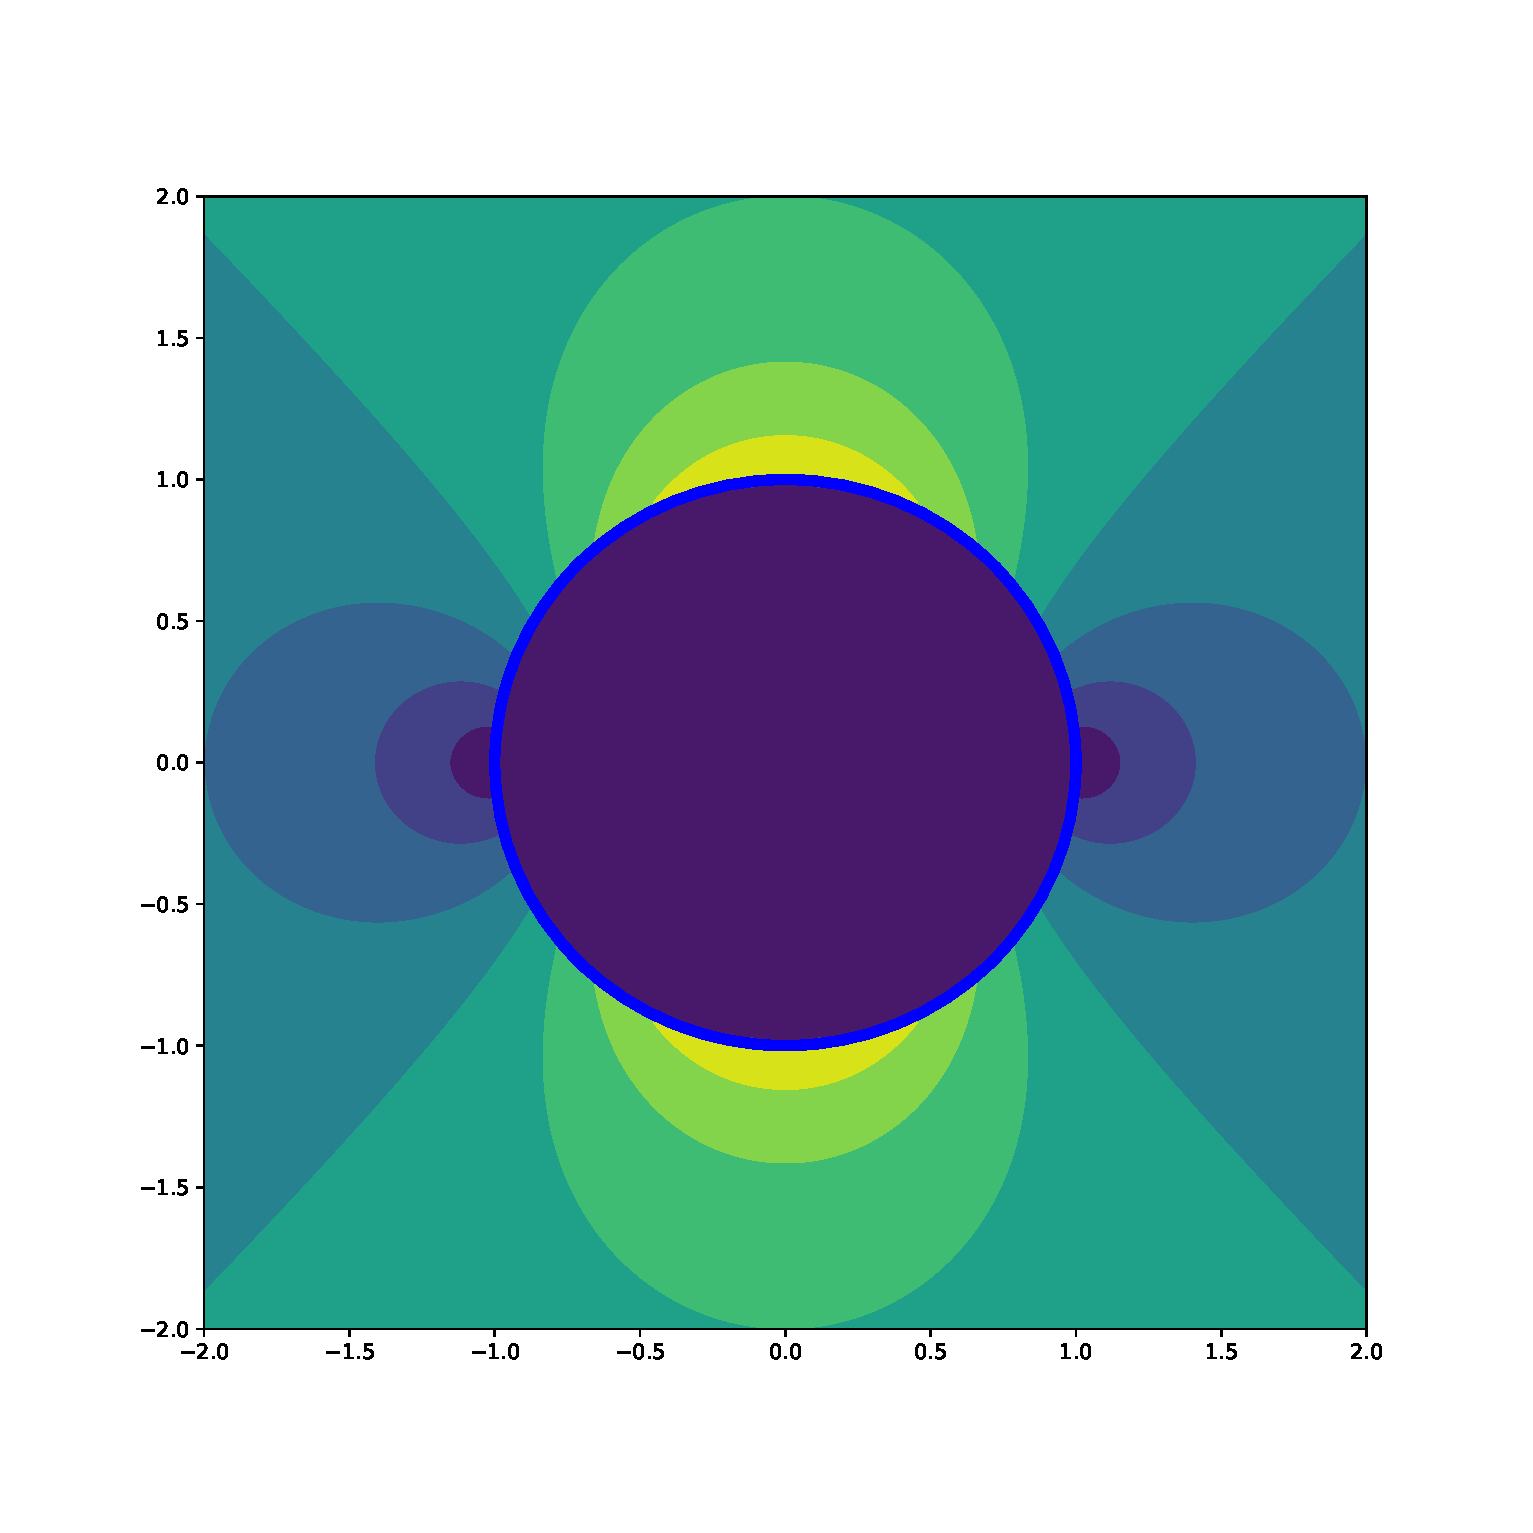
\includegraphics[width=0.4\linewidth]{figures/potential_flow_past_cylinder_vel}
  \caption{\label{fig:potential_flow_past_cylinder_vel}}
\end{figure}


\begin{figure}
  \centering
  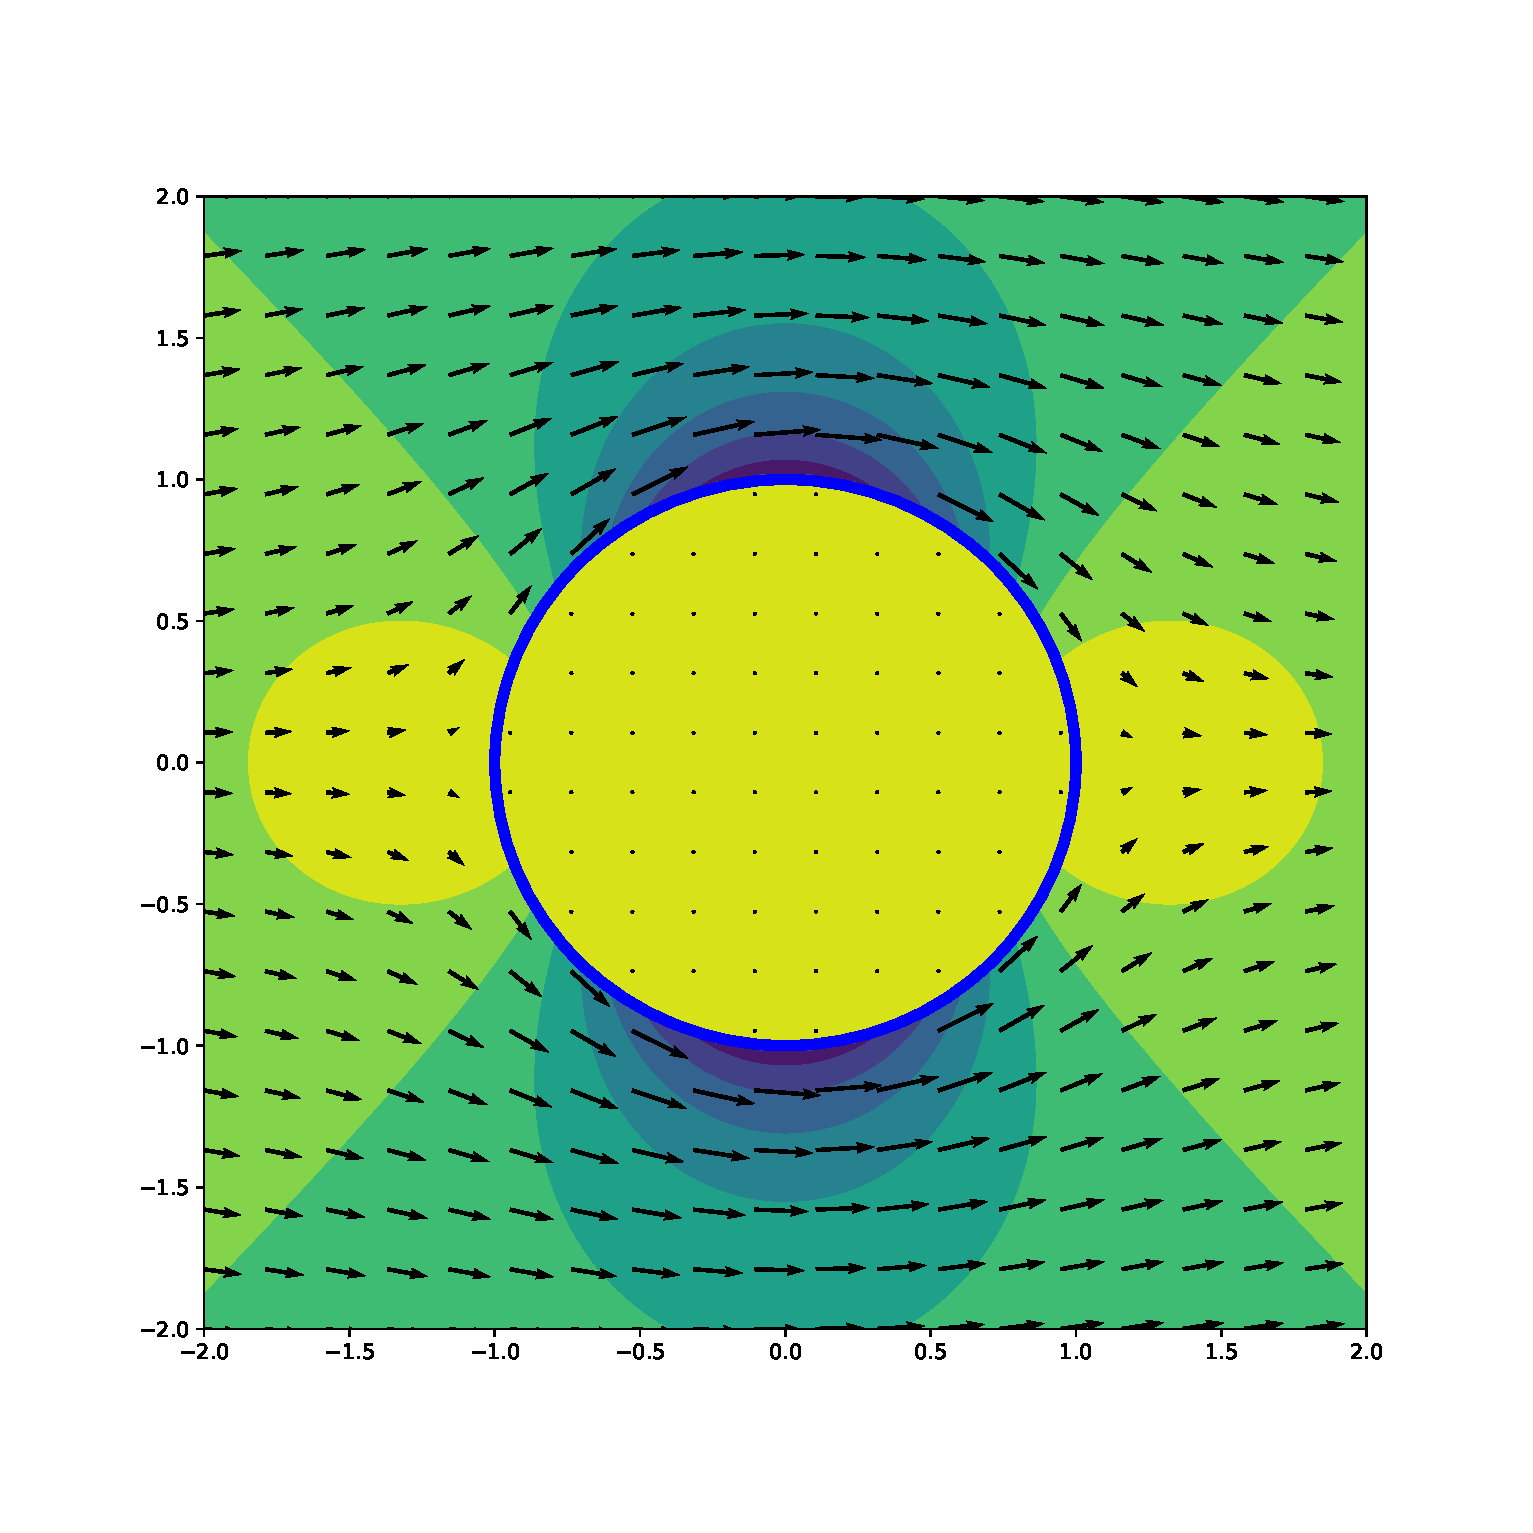
\includegraphics[width=0.4\linewidth]{figures/potential_flow_past_cylinder_vel_p}
  \caption{}%\label{fig:potential_flow_past_cylinder_vel}}
\end{figure}


The pressure field can be obtained from Bernoulli's principle:
\[
p= p_0 +  \frac{\rho}2  \left(u_0^2 - u^2 \right) ,
\]
and is plotted in
Fig. \ref{fig:potential_flow_past_cylinder_phi_p}. This Figure also
shows the potential field, to stress the difference between the
two. The velocity field does not simply ``goes from high to low
pressures'', except in those areas in which the two fields happen to
have similar gradients.

\begin{figure}
  \centering
  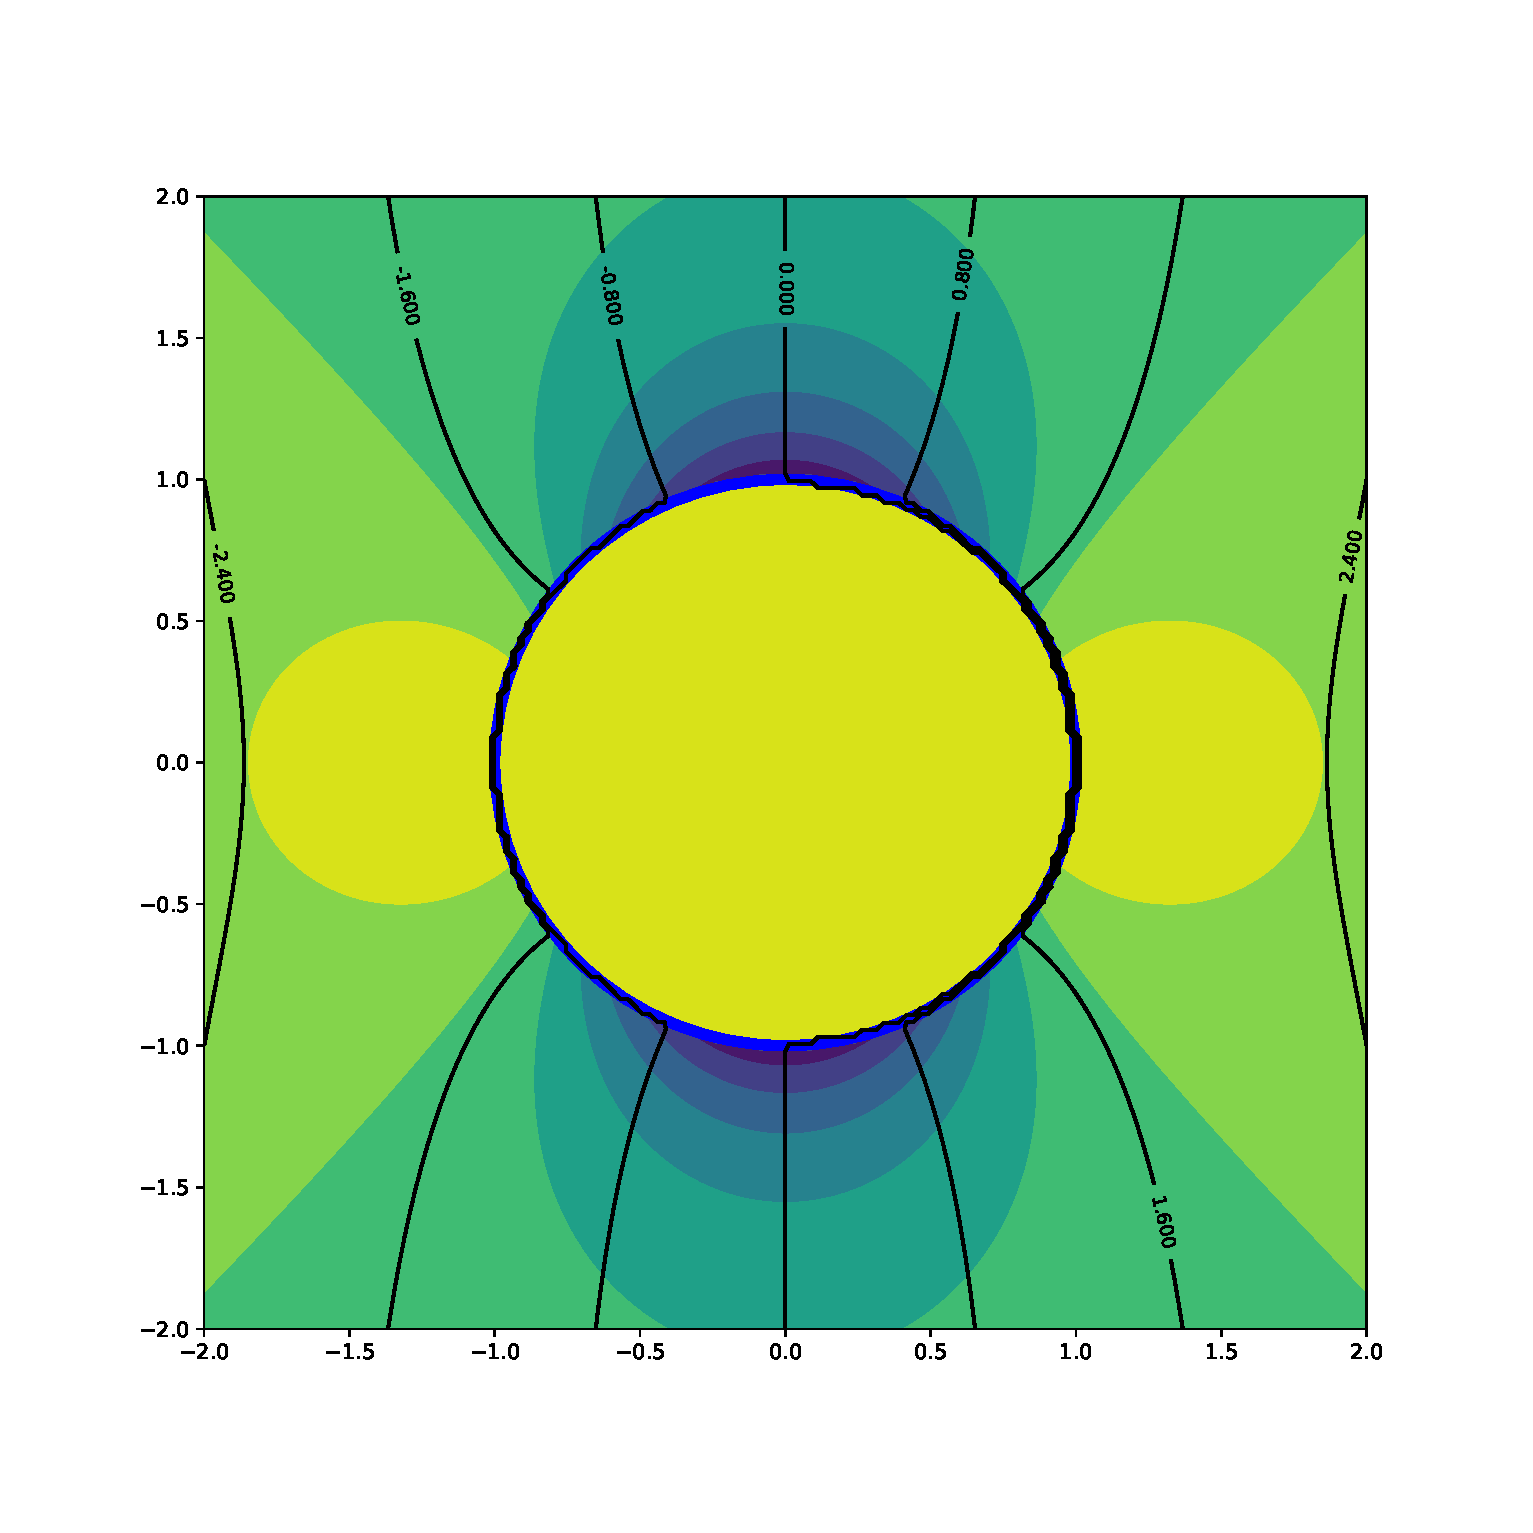
\includegraphics[width=0.4\linewidth]{figures/potential_flow_past_cylinder_phi_p}
  \caption{\label{fig:potential_flow_past_cylinder_phi_p}}
\end{figure}

The pressure field has a striking left-right symmetry. This of course
applied to its value at the surface. Since the pressure is the only
force this fluid may exert upon the cylinder, the consequence is that
the net force on it is exactly zero. The push it experiences towards
the right is exactly cancelled by the push back towards the
left. Therefore, the drag, which in this case is the net horizontal
force, is zero.

This striking result is known as d'Alembert's paradox, and marked a
historical chasm between theoretical fluid mechanics and applied
hydraulics. Indeed, the applied community could accept that the push
back may exist. Indeed, it had been hypothesized to be solely
responsible for objects moving even when not given a force in
Aristotelian physics. The effect is real, and is used regularly by
cyclist that may take advantage from it, by staying close to the back
of a moving vehicle. However, it is not acceptable to accept that it
should be exactly equal to the drag.

We now know that the crucial ingredient is the viscosity, which
manifests mathematically in a different boundary condition, such as
no-slip. This way, a real cylinder is dragged with the flow. We will
show later that it is easy to obtain the drag on a sphere in the limit
of high viscosity (a cylinder is not solvable due to another paradox,
as we will see.)

In case some mathematical justification is required, the pressure
at the surface on the cylinder is
\[
 p= p_0 + \frac12  u_0^2 \left(1 -  4   \sin^2(\theta) \right),
\]

Now, the drag is given by the net force in the $x$ direction. The
(vector) force due to pressure is:
\[
\mathbf{F} = \int_0^H \int_0^{2\pi}   p(\theta)  \bfn  R d\theta  dz ,
\]
where $p(\theta) \bfn \bhe_x R d\theta dz $ is the pressure force on a
differential surface of area $ R d\theta dz$. Now, the drag will be
its projection on the horizontal axis:
\[
D= \mathbf{F} \cdot \bhe_x = \int_0^H \int_0^{2\pi}
p(\theta) \cos(\theta) R d\theta dz .
\]
The integral is zero, since it consists of two terms. The first one
involves constant term. Of course, a constant pressure exerts no net
force, and mathematically:
\[
 \int_0^{2\pi} C \cos(\theta) d\theta = C  \int_0^{2\pi}  \cos(\theta) d\theta = 0 .
\]

The other term involves a $sin^2$ term. Now, this integral is also
zero:
\[
 \int_0^{2\pi}  \cos(\theta)  \sin^2(\theta) d\theta = 0 .
\]
qThe reason is that $\sin^2$ may be written as another constant term
and a term proportional to $\cos(2\theta)$. (To be precise,
$\sin^{2}\theta ={\frac {1-\cos(2\theta )}{2}}$.) Cosines form an
orthogonal basis: an integral of two different cosines over one period
will be zero. Unless they are the same cosine, when the integral is
$\pi$. To be precise, for integer $m$ and $n$:
\[
\frac{1}{2\pi} \int_0^{2\pi}  \cos(m \theta) \cos(n \theta)  d\theta = 
\begin{cases}
0 \quad \text{if } m\ne n \\
\frac12 \quad \text{if } m = n 
\end{cases} .
\]
(It is more elegant to divide by $2\pi$ to express the integral as a
mean value.) In fact, the previous result about the constant pressure
is a particular case in which $m=0$.

It is also interesting that such an integral involving a sine and a
cosine is always zero. This shows that the lift is always null:
\[
L= \mathbf{F} \cdot \bhe_x = \int_0^H \int_0^{2\pi}
p(\theta) \sin(\theta) R d\theta dz = 0
\]



\subsection{Streamlines}

For steady 2D flow, it is very convenient to introduce the stream
function $\psi$. It is defined such that its contour lines produce the
streamlines \index{streamline}, i.e. the lines the fluid particles
trace as they move. Upon some reflection, this means that its gradient
should always be perpendicular to the velocity:
\begin{equation}
  \label{eq:stream_perp_to_u}
  \bfu \cdot \nabla\psi = 0 .
\end{equation}
In steady flow, this means $d\psi/dt=0$, so the value of $\psi$ is
carried with the flow. This is at variance with the potential, whose
gradient is parallel to the velocity (it is indeed, the velocity
itself). Thus $\phi$ and $\psi$ are orthogonal functions, in the sense
that their gradients are.

The streamlines are important to visualize flows, in much the same way
as Faraday's field lines are for electromagnetic fields
(mathematically, they are equivalent). In computational fluid
dynamics, they are customarilly computed and plotted, by ``seeding''
points and integrating their motion following the velocity field.  A
fine point is that for unsteady flow, these streamlines are in general
different from the actual trajectories of fluid particles, which are
called ``pathlines'' \index{pathline}.


For steady flow, it is often convenient to define a vector potential
\index{vector potential} in much the same way as it is done for the
magnetic field in electromagnetism:
\begin{equation}
  \label{eq:vector_potential}
  \bfu = \nabla\times \bfA .
\end{equation}

The resulting velocity field will always be incompressible, since the
divergence of a curl is zero.

In the case of 2D, the choice for this vector potential is
\begin{equation}
  \label{eq:A_psi_2D}
  \bfA = \psi(x,y) \bhe_z ,    
\end{equation}
perpendicular to the plane, but dependent on the in-plane
coordinates. With this expression,
\begin{align*}
  u_x &=  \frac{\partial \psi}{\partial y} \\
  u_y &= -\frac{\partial \psi}{\partial x} ,
\end{align*}
and it is easy to check that this stream function indeed traces
stream-lines, since it complies with \ref{eq:stream_perp_to_u}.

In cylindrical coordinates \cite{wiki:del},
\begin{align*}
u_r &= \frac1r \frac{\partial \psi}{\partial \theta} \\
u_\theta &=   - \frac{\partial \psi}{\partial r} .
\end{align*}


\subsection{Streamlines around the cylinder}

With tha latter expression for the stream function, and from our
results for the velocity field, the $\psi$ field is found to be
\[
\psi = u_0 \left( r-{\frac {R^{2}}{r}}\right)\sin \theta .
\]
This method, of course, is working backwards from the known
solution. It is also possible to derive the velocity field from the
fact that $\psi$ satisfies Laplace's equation, plus the appropriate
boundary conditions, in a manner very similar to what has been done
for the potential (see Exercise \ref{ex:u_from_psi_cylinder}).

The contour lines of this field are shown in
Fig. \ref{fig:potential_flow_past_cylinder}.

\begin{figure}
  \centering
  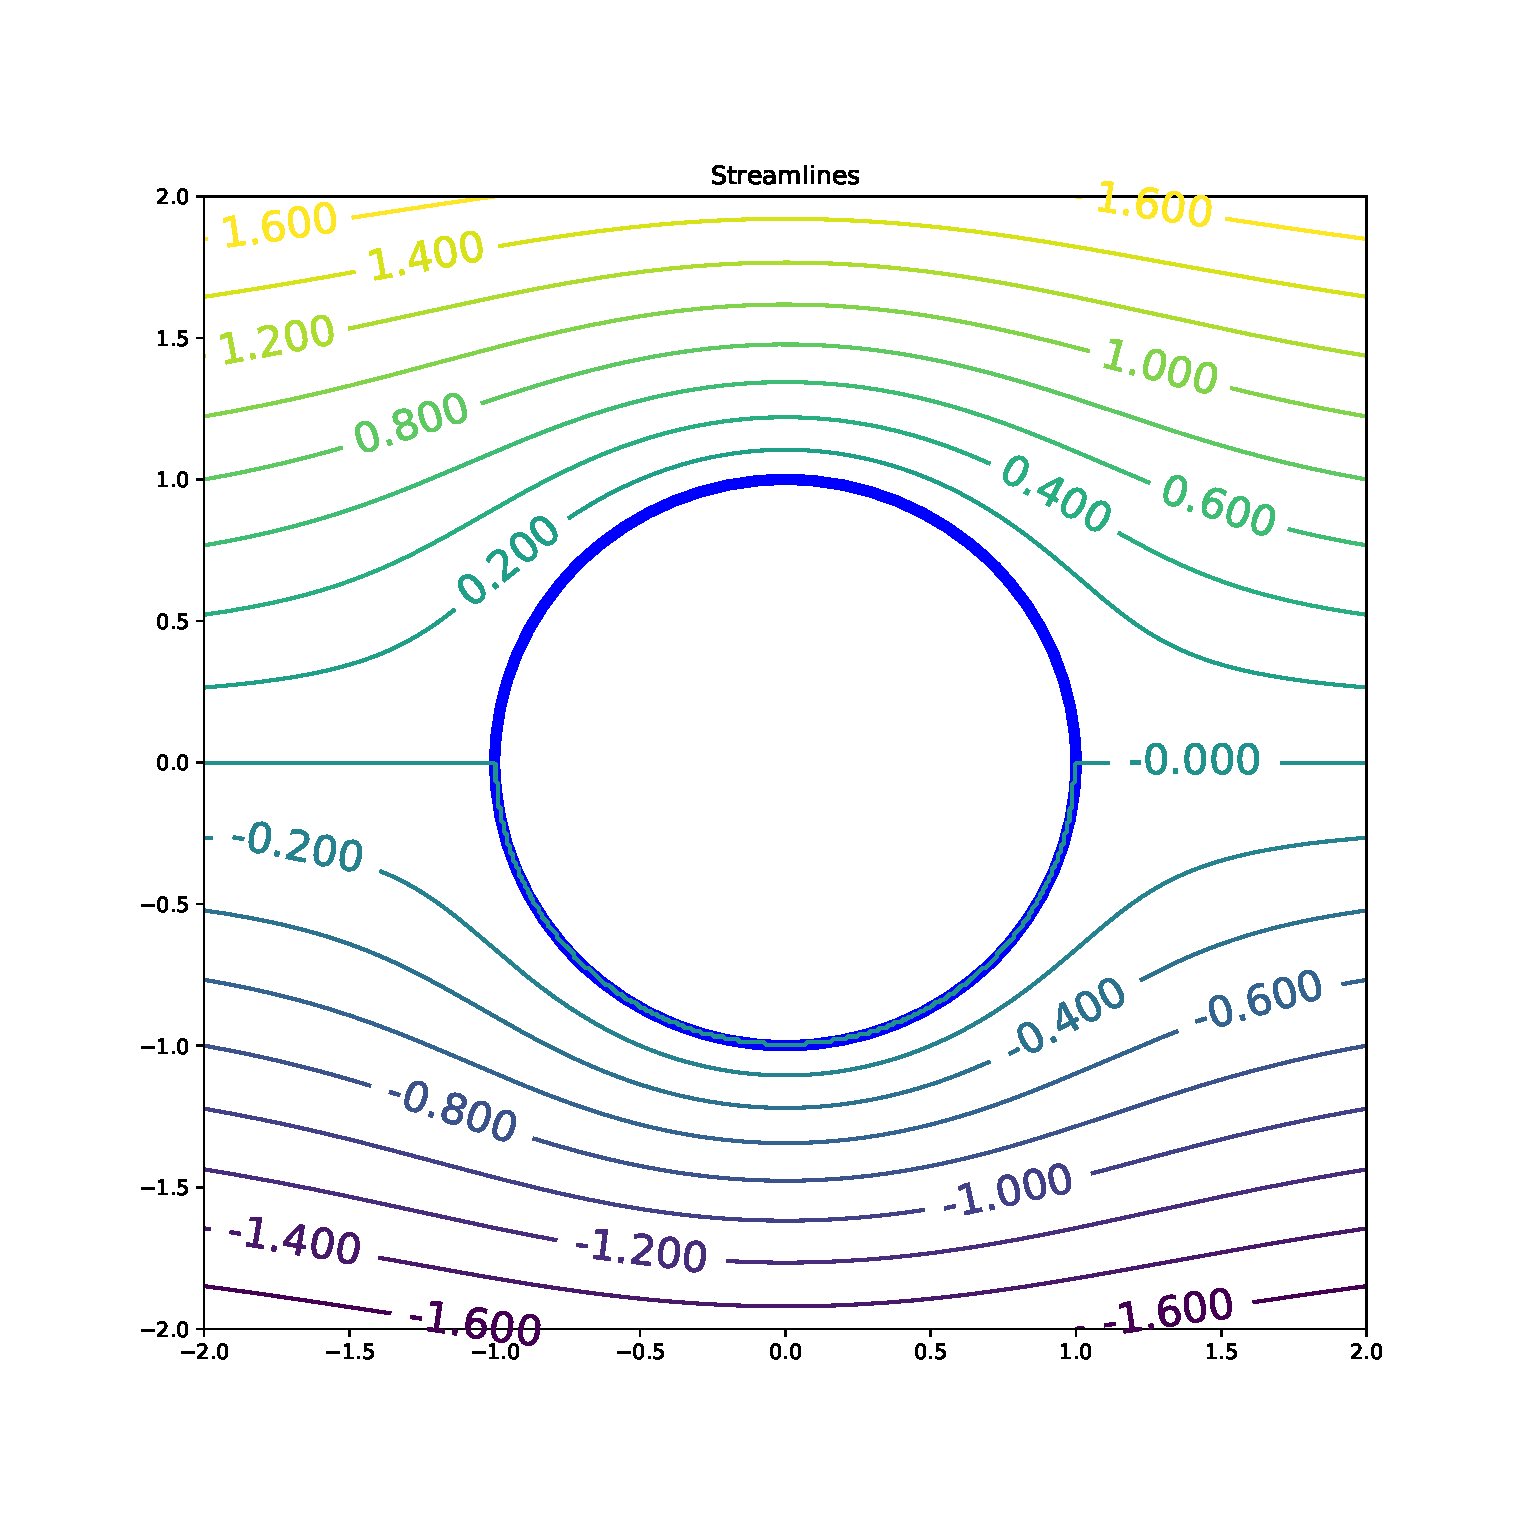
\includegraphics[width=0.4\linewidth]{figures/potential_flow_past_cylinder}
  \caption{\label{fig:potential_flow_past_cylinder}}
\end{figure}

Interestingly, the $\psi$ field is also a solution of Laplace's
equation, $\nabla^2 \psi=0$, as can be checked explicitely --- but
also from the identity for the curl of the curl
\cite{wiki:Vector_calculus_identities}:
\begin{equation}
  \label{eq:curl_of_curl}
  \nabla \times \left(\nabla \times \bfA \right)=
  \nabla (\nabla \cdot \mathbf {A} )-\nabla^2\bfA .
\end{equation}

Then, since the velocity field is curl-free:
\begin{equation}
  \label{eq:if_no_curl_then_stream_harmonic}
  0 = \nabla \times \bfu =
  \nabla (\nabla \cdot \mathbf {A} )- \nabla^{2}\mathbf {A} =
  - \bhe_z \nabla^{2} \psi,
\end{equation}
where we use the fact that the $\bfA$ field of \ref{eq:A_psi_2D} is
divergence-free.


There is also the intriguing fact that we may write
\[
\phi = u_0 \Re \left( z  + \frac{R^2}{z} \right) ,
\]
where $z=r e^{i\theta}$ is the complex number related to the $r$ and
$\theta$ coordinates. Then,
\[
\psi = u_0 \Im \left( z  + \frac{R^2}{z} \right) .
\]
%
I.e. both fields are the real and imaginary part of the same complex
function:
\[
f(z) = u_0 \left( z  + \frac{R^2}{z} \right)
\]

This is no coincidence, but a consequence of Cauchy-Riemann
equations: the real and imaginary part of a complex function are
harmonic (i.e. they satisfy Laplace's equation) and orthogonal. To be
more precise, the complex function must be analytic. The later
requirement is pretty general: it means the function must be
single-valued and and must have a derivative everywhere. The reader
may worry about the origin and the $1/z$ function. This is, however,
outside our domain, which ends when $r>R$. However, the fact that our
domain has this ``hole'' in it has some consequences, as we will see
next.


\subsection{Circulation and lift}

It turns out that, despite our previous claims of having found the
solution to the problem, this is not a unique solution%
\footnote{This is because our domain has a hole in it. Technically, it
  is not simply-connected. This means there is an additional parameter
  to fix the most general solution. This is called the ``winding
  number'', and is basically this section's $\Gamma$.}.
%
The most general one is given by
\[
 f(z) = u_0 \left( z + \frac{R^2}{z} \right)
 + \frac{i \Gamma}{2\pi} \log z \qquad
 \phi=\Re(f) \quad
 \psi=\Im(f) .
\]
I.e. we may add an additional term which is also analytic. The $i
\Gamma/(2\pi)$ factor is chosen for convenience, as will become
clear. Both $\phi$ and $\psi$ are still harmonic and orthogonal, since
$\log(z)$ is analytic. Notice $i \log(z)= i \log(r) - \theta$, so
$\phi$ contains a term that is just the polar angle, while $\psi$ will
include a $\log(r)$ term.

The resulting velocity field still complies with the boundary
conditions, since the resulting velocities:
\begin{align}
u_r     &=   u_0  \left[ 1 - \left( \frac{R}{r}\right)^2 \right] \cos(\theta) \\
u_\theta &=   u_0  \left[ 1 + \left( \frac{R}{r}\right)^2 \right] \sin(\theta) +\frac{\Gamma}{2\pi r} 
\end{align}
have an additional term which dies away far from the cylinder, while
the no-trespass condition at the surface is still respected (since the
radial velocity does not change at all).

The name of $\Gamma$ is ``circulation'', since
\[
\Gamma = \oint_C \bfu\cdot d\mathbf{l}
\]
for any contour around the cylinder \footnote{This makes the velocity
  field non-conservative, which is again allowed due to the domain
  being not simply-connected.}.

At the surface of the cylinder,
\[
u= u_\theta =   u_0  2 \sin(\theta) +\frac{\Gamma}{2\pi R} .
\]
The stagnation points then move away from their positions, to points given by
\[
\sin(\theta_\mathrm{st})  = \frac{\Gamma}{4\pi R u_0} .
\]
This has two solutions, of course, as long as the right-hand side is
between $-1$ and $1$. For values below or above, the points coalesce
into a single stagnation point that is outside the cylinder.

\begin{figure}
  \centering
  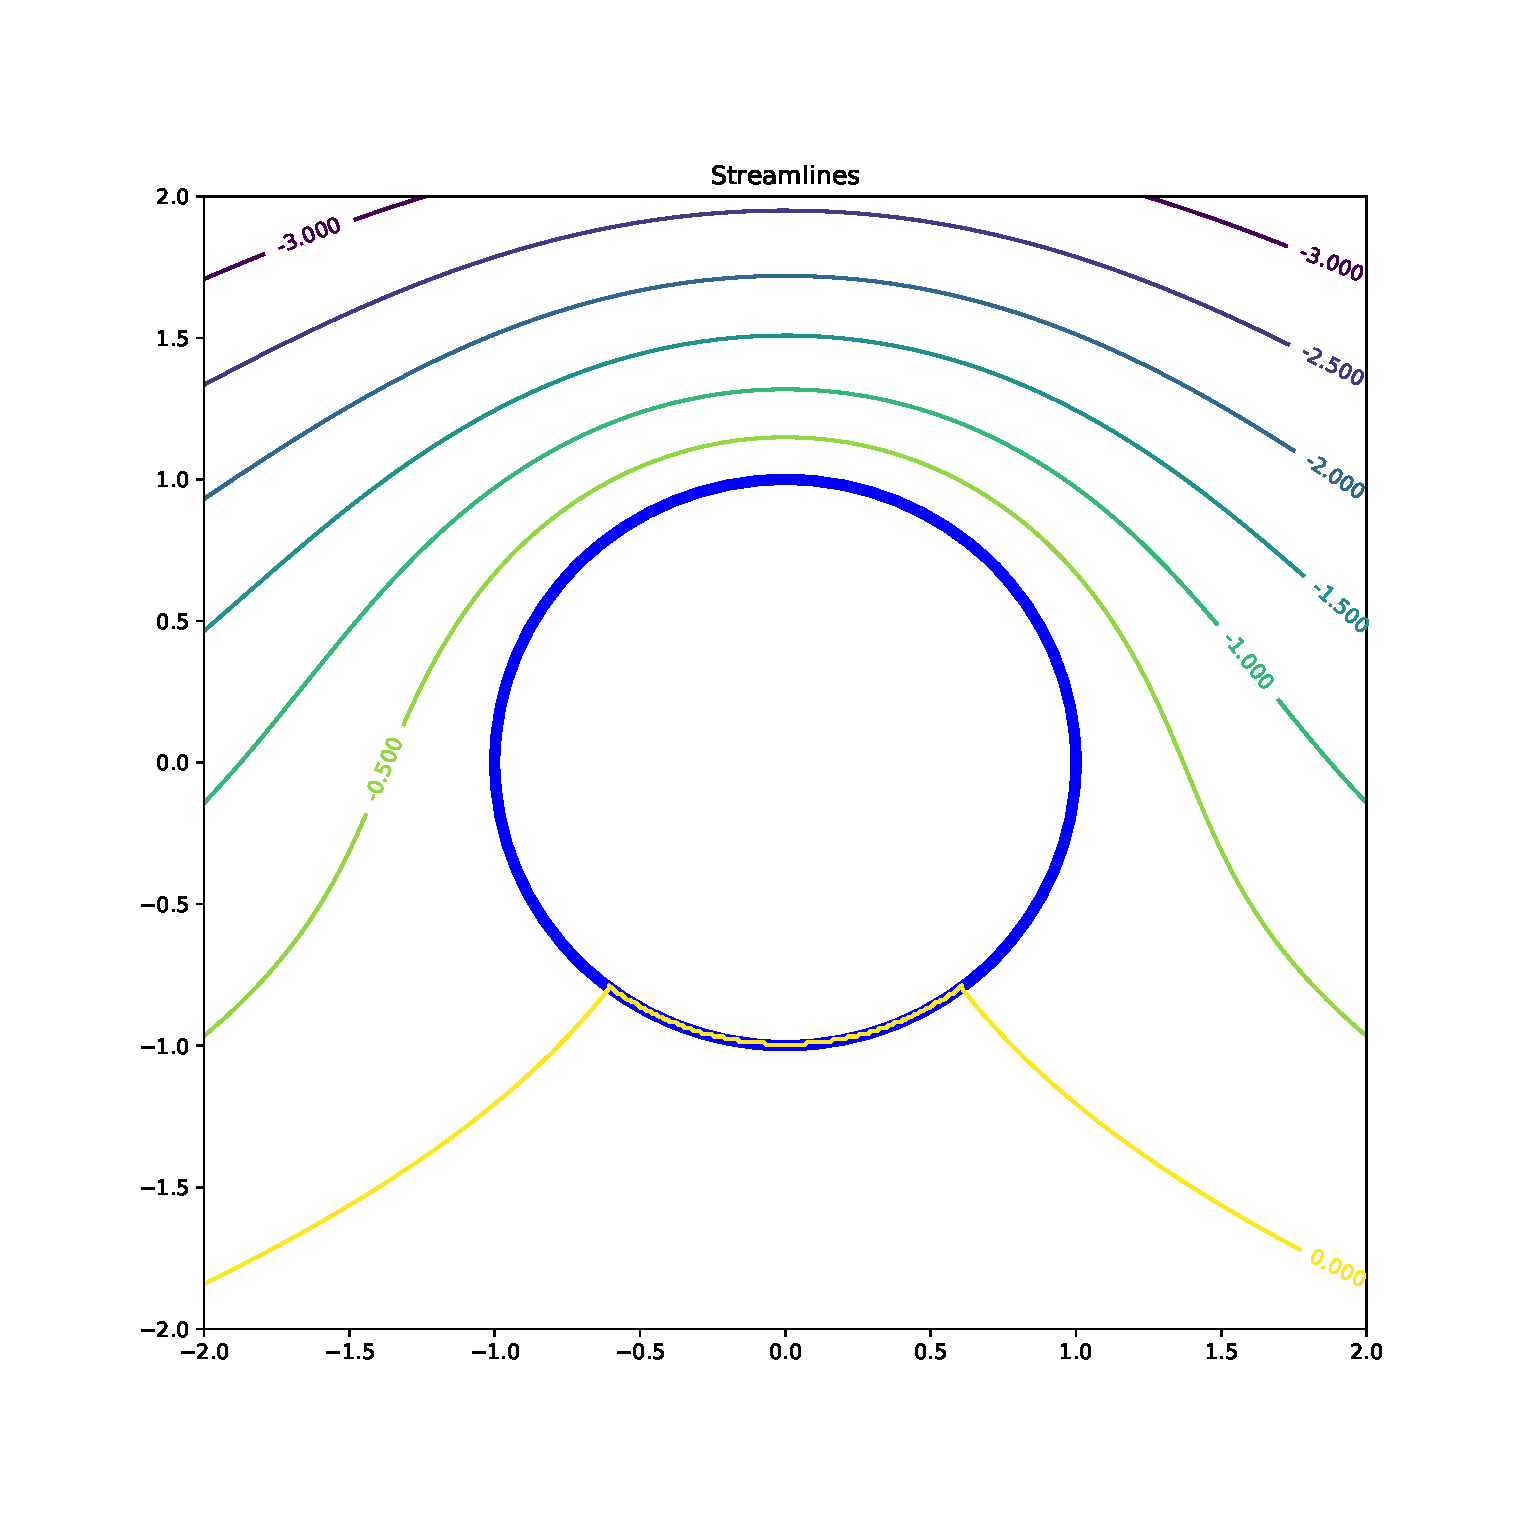
\includegraphics[width=0.4\linewidth]{figures/potential_flow_past_cylinder_rotating}
  \caption{\label{fig:}}
\end{figure}


This new velocity field does not solve d'Alambert's paradox, but it
does provide a lift, since the pressure at the surface is
\[
p= p_0 + \frac{\rho}2   \left(u_0^2 -  \left[ 2  u_0 \sin(\theta) - \frac{\Gamma}{2\pi R} \right]^2 \right) =
\ldots  2 \rho u_0   \frac{\Gamma}{2\pi R} \sin\theta ,
\]
where we single out the only term that can produce a contribution to the lift.

Now,
\begin{equation}
  \label{eq:lift_potential_cyl}
  L= \mathbf{F} \cdot \bhe_x = \int_0^H \int_0^{2\pi}
  p(\theta) \sin(\theta) R d\theta dz =
  2 L  \rho u_0  R  \frac{\Gamma}{2\pi R}   \int_0^{2\pi}  \sin^2(\theta) d\theta =
  H \rho u_0   \Gamma .
\end{equation}
Therefore, the lift per unit length is $L/H= \rho u_0 \Gamma$. It is
interesting that heavier fluids, high speeds and high $\Gamma$ produce
higher lift forces.

It turns out that this result for the lift is quite general, at least
for these kind of potential flows. It is known as the Kutta-Joukowski
Lift Theorem, and has been used for decades in aeronautics. The idea
is to map our solution for a cylinder to another, more wing-like,
shape, by some conformal transformations. These transformations, or
``mappings'', preserve the harmonicity of functions --- hence the
transformed $\phi$ and $\psi$ will still be solutions of Laplace's
equation. Historically, the best known mappings are the Joukowsky
K\'arm\'an–Trefftz transforms.

For a plane wing, it makes sense to relate circulation and lift, since
this captures, in a way, the fact that the velocity is higher at the
top of the wing, lower below, so the net circulation is non zero. (Of
course, this cannot hold right at the surface of an actual wing, since
the velocity there will be zero. But this can be measured somewhat
further away, beyond a boundary layer.) For a cylinder, this makes
little sense, but this picture is sometimes used to explain the Magnus
effect. This causes a rotating cylinder to bend as it moves across a
fluid. This is used (for spheres) in sports, such as tennis, golf and
football. Also, for cylinder-like rotors in ``rotor ships,'' which use
the Magnus effect for propulsion.

As an aside, if we move along with the plane, or ship, we will not see
those velocity fields. The horizontal component should be avoided in
every equation, and the resulting velocity looks different. This is
shown in Fig. \ref{fig:potential_flow_past_cylinder_moving}, for the
flow past a cylinder with and without circulation. It is seen that,
for an observoer moving with the cylinder, the surrounding fluid is
pushed from the fore, and moved around towards the aft (where it
pushes our vehicle, magically making our journey a costless one!).

\begin{figure}
  \centering
  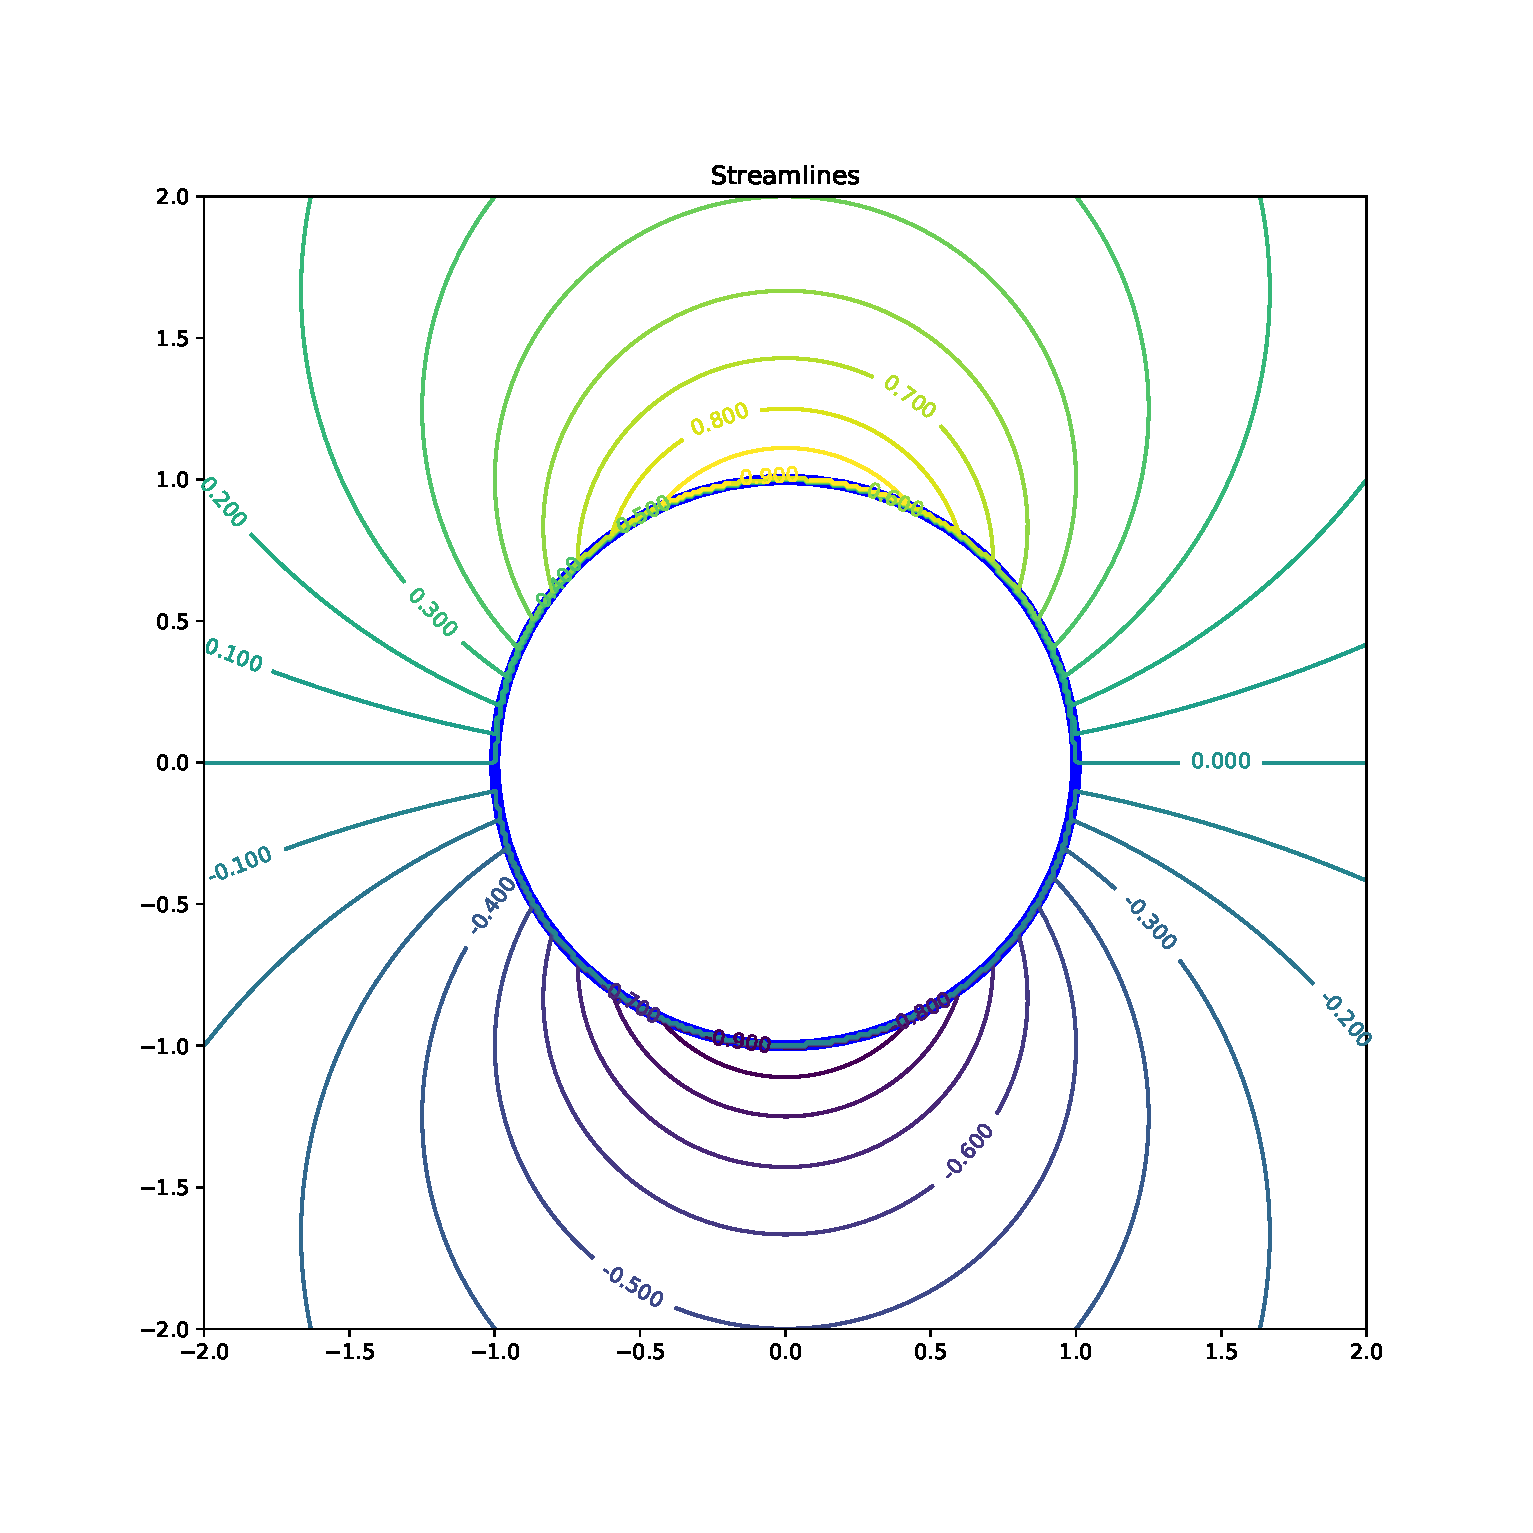
\includegraphics[width=0.4\linewidth]{figures/potential_flow_past_cylinder_moving}
  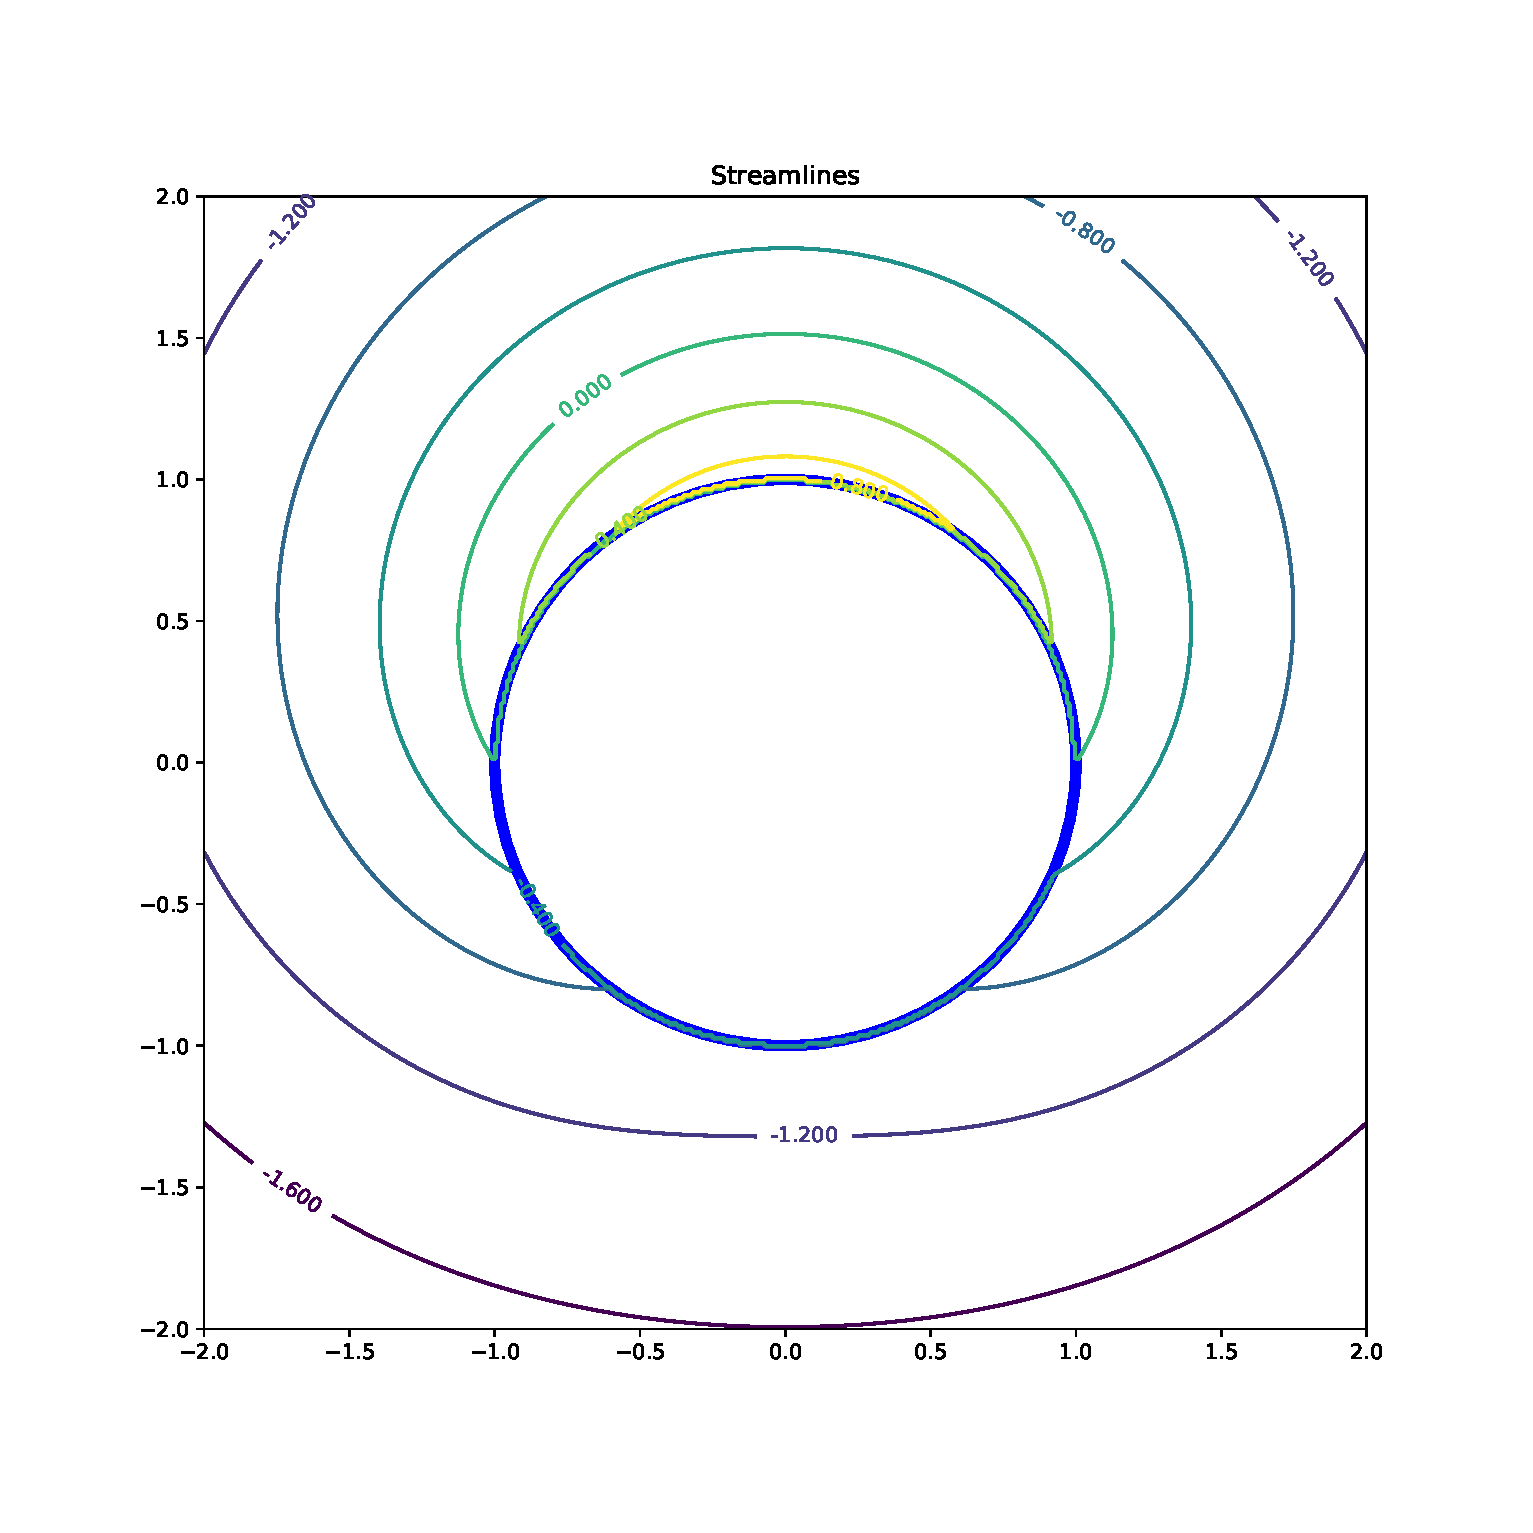
\includegraphics[width=0.4\linewidth]{figures/potential_flow_past_cylinder_rotating_moving}
  \caption{\label{fig:potential_flow_past_cylinder_moving}}
\end{figure}


\section{Flow past a sphere}

With the same assumption of potential flow as in the cylinder, the
axisymmetric flow past a sphere may be tackled by using the potential,
which should satisfy Laplace's equation, plus these boundary
conditions:
\[
  \phi (r\to \infty) \to u_0 z = u_0 r \cos\theta \qquad
  u_r(r=R) =\left. \frac{\partial \phi}{\partial r} \right|_{r=R} = 0 .
\]
Spherical coordinates \index{spherical coordinate system} are used:
$r$ is the distance to the origin, $\theta$ is the polar angle (angle
with the $z$ axis), and the azimuthal angle (angle around the $z$
axis), here absent due to symmetry, is $\phi$ %.
\footnote{This naming convention is the most common in physics, and is
  pecified by ISO standard 80000-2:2009, and earlier in ISO 31-11
  (1992). However, the name of the two angles is often reversed,
  specially in mathematics. The advantage of the latter is that
  $\theta$ then retains the same name as in 2D polar coordinates.}.


Similarly to the cylinder, let us try a function
\[
\phi =  \left( u_0 r  + f(r) \right) \cos(\theta)  .
\]

By using the expression of the Laplacian in spherical coordinates
\cite{wiki:del}, we soon come to the conclusion that $f(r)= A/r $ in
order Laplace's equation be satisfied. This function also vanishes as
$r$ gets large, as it should. With the no-trespassing condition for the
velocity the value of $A$ may be found out.

The final result is
\[
  \phi(r,z) = u_0 r
  \left[
    1 +
    \frac12 \left( \frac{R}{r}\right)^3
  \right] \cos\theta .
\]
From its gradient we get the velocity field:

\begin{align*}
u_r &=  u_0
  \left[
    1 -
      \left(\frac{R}{r}\right)^3
  \right] \cos\theta \\
u_\theta &=  -u_0
  \left[
    1 + \frac12
      \left(\frac{R}{r}\right)^3
  \right] \sin\theta
\end{align*}


\subsection{Streamlines past a sphere}

For axisymmetric flows, streamlines may be defined on a plane, since
the resulting flow does not depend on the azimuthal angle (the angle
around the axis of symmetry, which is $z$). However, these are not 2D
flows, and the equations are more involved.

In this case, the velocity field depends only on the other two
coordinates. In spherical coordinates,
\[
  \bfu = \bfu(r,\theta) .
\]

The vector potential may still be thought of as ``perpendicular'' to the other
two coordinates. In spherical coordinates:
\[
  \bfA = A \bhe_\phi ,
\]
i.e. it is purely azimuthal. It is also divergence-free, so that is
satisfies Laplace's equation for a curl-free flow, by the argument
exactly as in Eq. \ref{eq:if_no_curl_then_stream_harmonic}.

However, the choice of $A=\psi$ does \emph{not} result in the correct
stream-line behavior of Eq.  \ref{eq:stream_perp_to_u}.

In axisymmetric flow,
\[
  \divu =
  {1 \over r^2}{\partial \left( r^2 u_r \right) \over  \partial r} +
  {1 \over r\sin\theta}{\partial \over \partial  \theta} \left( u_\theta\sin\theta \right) ,
\]
but an equivalent expression is
\[
  \divu =
  {\partial \left( r^2 u_r \sin\theta \right) \over  \partial r} +
  {\partial \left( r u_\theta\sin\theta \right)  \over \partial  \theta} .
\]
The curl in spherical coordinates is
\begin{align}
  u_r     &= \frac {1}{r\sin \theta }
            \frac{ \partial  \left( A  \sin \theta \right) }{\partial \theta }  \\
  u_\theta &= -\frac1{r} \frac{\partial (rA) }{\partial r} .
\end{align}
Therefore,
\[
  \divu =
  {\partial\over\partial r} \left( r
      \frac{ \partial  \left( A  \sin \theta \right) }{\partial \theta }
    \right)  -
  {\partial \over \partial  \theta}  \left(
      \frac{\partial (rA) }{\partial r} 
      \sin\theta \right)  .
\]
Continuity is therefore trivially satisfied with the choice
\begin{equation}
  \label{eq:Stokes_stream_spherical}
  \bfA = \frac{\psi(r,\theta)}{r \sin\theta } \bhe_\phi .    
\end{equation}
%
This $\psi$ is called ``Stokes stream function''\index{Stokes stream
  function}, since there are differences with the 2D stream function
  (traditionally called ``Lagrange stream function''.)

Appling the curl expression, we find
\begin{equation}
  \label{eq:u_from_psi_spherical}
  \begin{split}
    u_r     &=  \frac1{r^2 \sin\theta} \frac{\partial \psi}{\partial \theta} \\
    u_\theta &= -\frac1{r   \sin\theta} \frac{\partial \psi}{\partial r} .
  \end{split}
\end{equation}
%
There may be an additional azimuthal $u_\phi$ velocity component
which cannot be obtained from $\psi$ (see Ex. \ref{ex:azimuthal_velocity}).


For completeness, in cylindrical coordinates the appropriate
expression is
\[
  \bfA = \frac{\psi(\rho, z)}{ \rho } \bhe_\phi ,
\]
where $\rho$ is the distance to the $z$ axis. Notice this is the same
expression as in spherical coordinates, since
$\rho=r\sin\theta$. There is a reason for this, as explained in
Ref. \cite{batchelor} p. 78.


The resulting velocity field is
\begin{equation*}
  \begin{split}
    u_\rho   &= - \frac1{\rho} \frac{\partial \psi}{\partial z} \\
    u_z     &=   \frac1{\rho} \frac{\partial \psi}{\partial \rho}
  \end{split}
\end{equation*}


For the flow around a sphere, the resulting stream function is then
found to be
\begin{equation}
  \label{eq:potential_sphere_stream}
  \psi(r,\theta) = \frac12 u_0 r^2
  \left[
    1 -
    \left(\frac{R}{r}\right)^3
  \right] \sin^2\theta .
\end{equation}
Again, this is found by working backwards from the known solution.
See Exercise \ref{ex:u_from_psi_sphere}) to derive the velocity field
from $\psi$.

In Fig. \ref{fig:potential_streamlines_sphere} these streamlines are
plotted. The corresponding streamlines for the flow as seen from the
sphere are in Fig. \ref{fig:potential_streamlines_moving_sphere}.

\begin{figure}
  \centering
  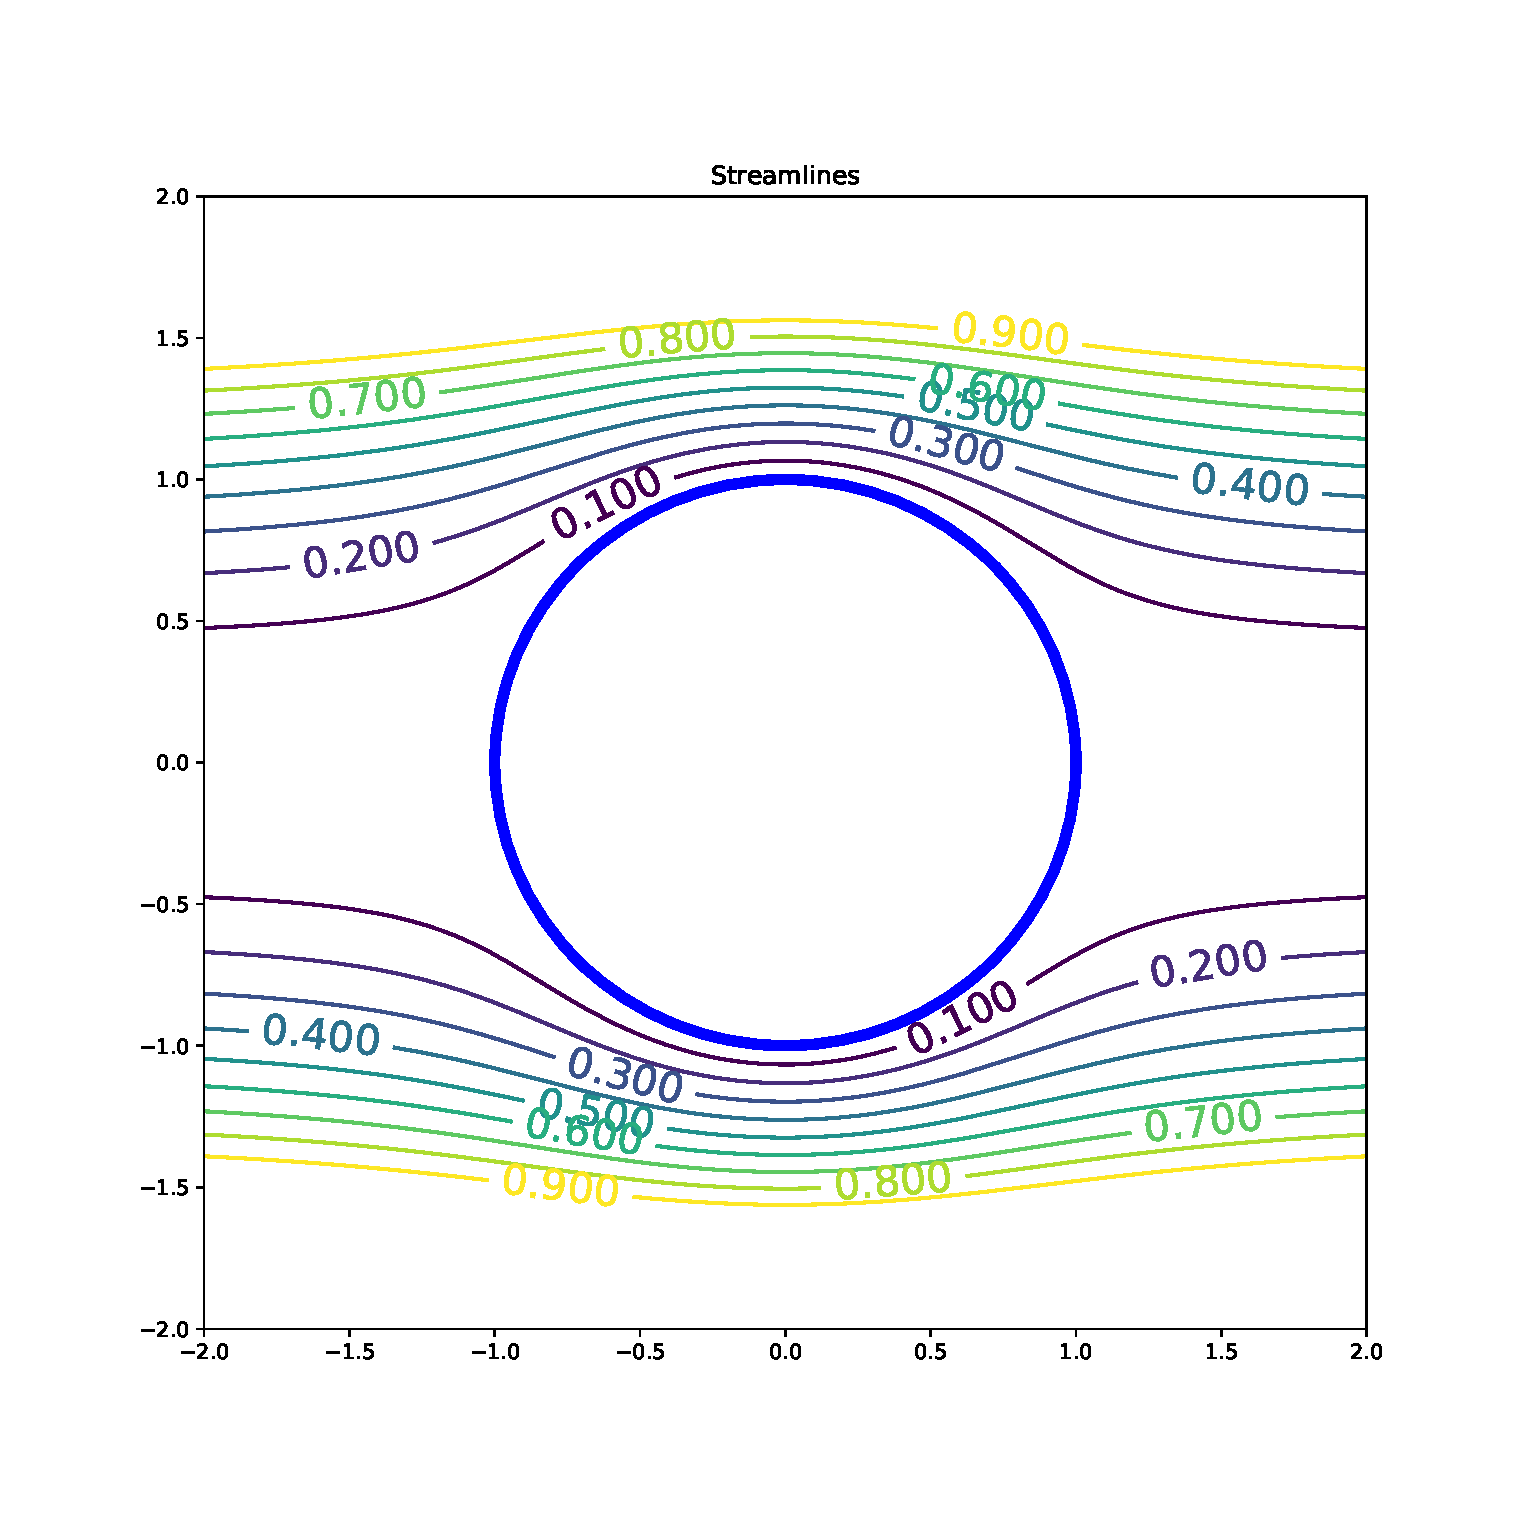
\includegraphics[width=0.4\linewidth]{figures/potential_flow_past_sphere}
  \caption{\label{fig:potential_streamlines_sphere} Streamlines of
    the potential flow past sphere}
\end{figure}



\begin{figure}
  \centering
  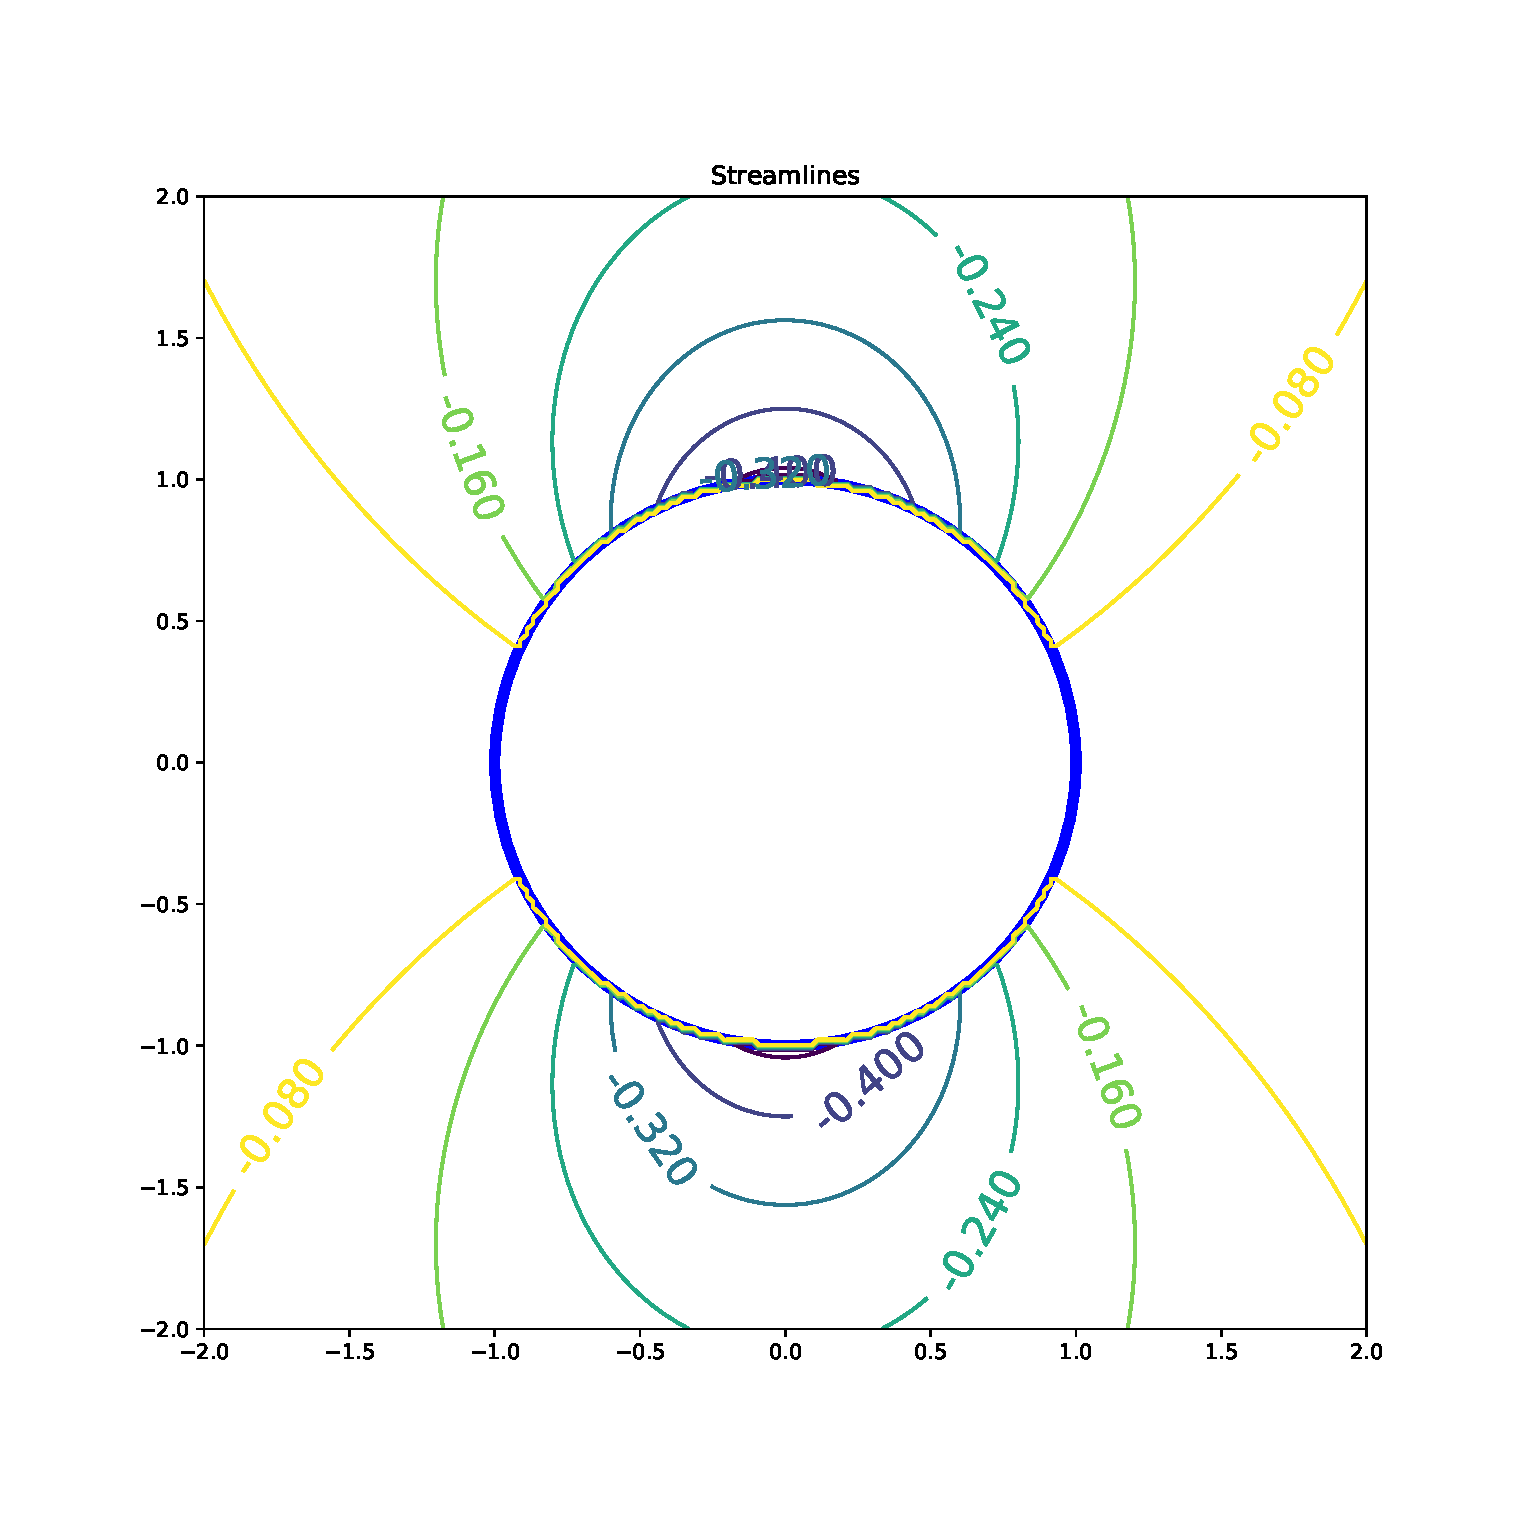
\includegraphics[width=0.4\linewidth]{figures/potential_flow_past_sphere_moving}
  \caption{\label{fig:potential_streamlines_moving_sphere}}
\end{figure}


\subsection{Exercises}

\begin{itemize}
\item \label{ex:u_from_psi_cylinder} Derive the velocity field for
  potential flow around a cylinder from $\psi$, solving Laplace
  equation for this field, plus the appropriate boundary conditions.
  
\item \label{ex:u_from_psi_sphere} Derive the velocity field for
  potential flow around a sphere from $\psi$, solving Laplace equation
  for this field with the appropriate boundary conditions. Use the
  fact that Laplace equation $\nabla^2 \bfA = 0$ may be written for
  $\psi$ using this identity:
  \begin{equation}
    \label{eq:psi_eq_from_A}
    \nabla^2 \left(  \frac{\psi(r,\theta)}{r \sin\theta } \bhe_\phi \right) =
    \frac{1}{r \sin\theta } 
    \left(
      \frac{\partial^2  }{\partial r^2} +
      \frac{1}{r^2} \left[
        \frac{\partial^2 }{\partial \theta^2} - 
        \cot(\theta) \frac{\partial }{\partial \theta}
      \right]
    \right) \psi \bhe_\phi .
  \end{equation}

\item Prove the previous identity. Notice that $\bfA$ is a vector
  field, so one need to apply the expression for the vector Laplacian
  of e.g. \cite{wiki:del}. The expressions are not so bad since the
  field is azimuthal only, and dependent on the other two components:
  $ \bfA = A(r,\theta) \bhe_\phi$.

\item Repeat the previous two calculation using cylindrical
  coordinates. Prove that
  \begin{equation}
    \label{eq:psi_eq_from_A_cyl}
    \nabla^2 \left(  \frac{\psi(\rho ,z) }{\rho} \bhe_\phi \right) =
    \frac{1}{ \rho } 
    \left(
      \frac{\partial^2  }{\partial \rho^2} -
      \frac{1}{ \rho } 
      \frac{\partial  }{\partial \rho} +
      \frac{\partial^2  }{\partial z^2}
    \right) \psi \bhe_\phi .
  \end{equation}
  

\item \label{ex:azimuthal_velocity}) Prove that the velocity may
  indeed have an azimuthal component for axisymmetric flow. Begin by
  writing down the expressions for the divergence and the curl in
  spherical coordinates, and neglecting all variation on the azimuthal
  angle, allowing for the possibility that the vector potential may
  have all three components, not just than $A_\phi$.  This result in a
  $u_\phi$ velocity component that can have basically any expression
  as far as continuity equation is concerned, since this is always
  satisfied




\end{itemize}



